
\documentclass[12pt,final]{article}
\usepackage{amsmath}
\usepackage{amssymb}
\usepackage{graphicx}
\usepackage{epsfig}
\usepackage{algorithm}
\usepackage{program}

\textwidth 6in
\textheight 8.5in
\oddsidemargin 0.25in
\evensidemargin 0.25in
\topmargin -.25in

%%%%%%%%%%%%%%%%%%%%%%%%%%%%%%%%%%%%%%%%%%%%%
\title{Sierra Low Mach Module Nalu: Verification manual}


\author{Stefan P. Domino\\
	Thermal Fluids Computation Engineering Sciences \\		
	Sandia National Laboratories\footnote {Sandia is a multiprogram laboratory operated by Sandia Corporation, a
        Lockheed Martin Company, for the United States Department of Energy
        under Contract DE-AC04-94AL850000}\\	
	Albuquerque, NM
        Email:  spdomin@sandia.gov\\
        Phone:  505-284-4317}

%==============================================================================
\begin{document}
\maketitle
This write-up represents a formal verification plan for the low Mach
number thermal fluids code, Nalu. 

%%%%%%%%%%%%%%%%%%%%%%%%%%%%%%%%%%%%%%%%%%%%%%%%%%%%%%%%%
\section{Introduction}
\label{s:intro}
%%%%%%%%%%%%%%%%%%%%%%%%%%%%%%%%%%%%%%%%%%%%%%%%%%%%%%%%%
Intro is the theory manual.

%%%%%%%%%%%%%%%%%%%%%%%%%%%%%%%%%%%%%%%%%%%%%%%%%%%%%%%%%
\section{Numerical scheme and code base}
\label{s:cvfem}
%%%%%%%%%%%%%%%%%%%%%%%%%%%%%%%%%%%%%%%%%%%%%%%%%%%%%%%%%
Nalu is the code base.

%%%%%%%%%%%%%%%%%%%%%%%%%%%%%%%%%%%%%%%%%%%%%%%%%%%%%%%%%
\section{Methodology for Testing}
\label{s:method}
%%%%%%%%%%%%%%%%%%%%%%%%%%%%%%%%%%%%%%%%%%%%%%%%%%%%%%%%%
The methodology used to evaluate the accuracy of each proposed
scheme will be the method of manufactured solutions.

The objective of code verification is to reveal coding mistakes that affect the order 
of accuracy and to determine if the governing discretized equations are being solved correctly.
Quite often, the process of verification reveals algorithmic issues that would otherwise remain 
unknown.

In practice, a variety of comparison techniques exist for verification. For example, 
benchmark and code-to-code comparison are not considered rigorous due to the errors
that exist in other code solutions, such as from discretization and iteration. Analytic 
solutions and the method of manufactured solutions remain the most powerful methods for 
code verification, since they provide a means to obtain quantitative error estimations in 
space and time.

Roache has made the distinction between 
code verification and calculation 
verification, where calculation verification involves grid refinement required for every 
problem solution to assess the magnitude, not order, of the discretization error. Discretization
error, distinguished from modeling and iteration errors, is defined as the difference between
the exact solution to the continuum governing equations and the solution to the algebraic 
systems representation due to discretization of the continuum equations. The order of accuracy
can be determined by comparing the discretization error on successively refined grids. Thus, it
is desirable to have an exact solution for comparision to determine the discretization errors.


%%%%%%%%%%%%%%%%%%%%%%%%%%%%%%%%%%%%%%%%%%%%%%%%%%%%%%%%%
\section{2D Unsteady Uniform Property: Convecting Decaying Taylor Vortex}
%%%%%%%%%%%%%%%%%%%%%%%%%%%%%%%%%%%%%%%%%%%%%%%%%%%%%%%%%

Verification of first-order and second-order temporal accuracy for the
CVFEM and EBVC formulation in Nalu is performed using the method of manufactured 
solution (MMS) technique. For the unsteady isothermal, uniform laminar physics set,
the exact solution of the convecting, decaying Taylor vortex is used.

\begin{equation}
  u = u_o - cos(\pi(x-u_ot)) sin(\pi(y-v_ot))e^{-2.0\omega t}
\label{advConvTV_u}
\end{equation}

\begin{equation}
  v = v_o + sin(\pi(x-u_ot)) cos(\pi(y-v_ot))e^{-2.0\omega t} 
\label{advConvTV_v}
\end{equation}

\begin{equation}
  p = -\frac{p_o}{4}(cos(2\pi(x-u_ot)) + cos(2\pi(y-v_ot)))e^{-4\omega t}
\label{advConvTV_p}
\end{equation}

In this study, the constants $u_o$, $v_o$, and $p_o$ are all assigned values of $1.0$,
and the viscosity $\mu$ is set to a
constant value of $0.001$. The value of $\omega$ is $\pi^2\mu$. This particular viscosity value 
results in a maximum cell reynolds number of twenty.  

\subsection{Temporal Order Of Accuracy Results}
The temporal order of accuracy for the first order backward Euler and second order BDF2
are outlined in Figure~\ref{fig:fo4thTstep} and Figure~\ref{fig:fo4thTstep}. Each of these
simulations used a hybrid factor of zero to ensure pure second order central usage. A
fixed Courant number of two was used for each of the three meshes (100x100, 200x200 and 400x400).
The simulation was run out to 0.2 seconds and L2 error norms were computed. The standard
fourth order pressure stabilization scheme with time step scaling is used. This scheme is also
known as the standard pressure-free approximate pressure projection scheme.

Two other pressure projection schemes have been evaluated in this study. Each represent a 
simplification of the standard pressure projection scheme. Figure~\ref{fig:hybridTstep} outlines
two projection schemes: the first is when the projected nodal graidnet is lagged and the 
second is the classic pressure-free pressure approximate projection scheme with second
order pressure stabilization. The error plots demonstrate that lagging the projected nodal
gradient for pressure retains second order accuracy. However, as expected the pressure
free pressure projection scheme is conformed to be first order accurate.

The 
Steady Taylor Vortex will be used to verify the spatial accuracy for the full set of advection
operators supported in Nalu.
 
\begin{figure}
\centerline{\includegraphics[width=0.6\textwidth]{figures/convTaylorVortexFO.eps}}
\caption{Error norms as a function of timestep size for the $u$ and $v$
component of velocity using fourth order pressure stabilization with timestep scaling, backward Euler}
\label{fig:fo4thTstep}
\end{figure}

\begin{figure}
\centerline{\includegraphics[width=0.6\textwidth]{figures/convTaylorVortexSO.eps}}
\caption{Error norms as a function of timestep size for the $u$ and $v$
component of velocity using fourth order pressure stabilization with timestep scaling, BDF2}
\label{fig:so4thTstep}
\end{figure}

\begin{figure}
\centerline{\includegraphics[width=0.6\textwidth]{figures/convTaylorVortexSO_ElemLagElemPf.eps}}
\caption{Error norms as a function of timestep size for the $u$ and $v$
component of velocity using the lagged projected nodal pressure gradient and pressure-free pressure projection scheme; all with with timestep scaling, BDF2}
\label{fig:hybridTstep}
\end{figure}

\section{Future work}
%%%%%%%%%%%%%%%%%%%%%%%%%%%%%%%%%%%%%%%%%%%%%%%%%%%%%%%%%

%%%%%%%%%%%%%%%%%%%%%%%%%%%%%%%%%%%%%%%%%%%%%%%%%%%%%%%%%
\section{Conclusions}
%%%%%%%%%%%%%%%%%%%%%%%%%%%%%%%%%%%%%%%%%%%%%%%%%%%%%%%%%

%%%%%%%%%%%%%%%%%%%%%%%%%%%%%%%%%%%%%%%%%%%%%%%%%%%%%%%%%
%%%%%%%%%%%%%%%%%%%%%%%%%%%%%%%%%%%%%%%%%%%%%%%%%%%%%%%%%
\section*{Acknowledgments}
%%%%%%%%%%%%%%%%%%%%%%%%%%%%%%%%%%%%%%%%%%%%%%%%%%%%%%%%%
Sandia is a multiprogram laboratory operated by Sandia Corporation, a Lockheed Martin Company, for the United States Department of Energy under Contract DE-AC04-94AL850000.

\end{document}

